\subsection{Joint Performance from Fingerprint and Finger Knuckle Images\label{joint-performance}}

\begin{figure*}
    \centering
    \subfloat[]{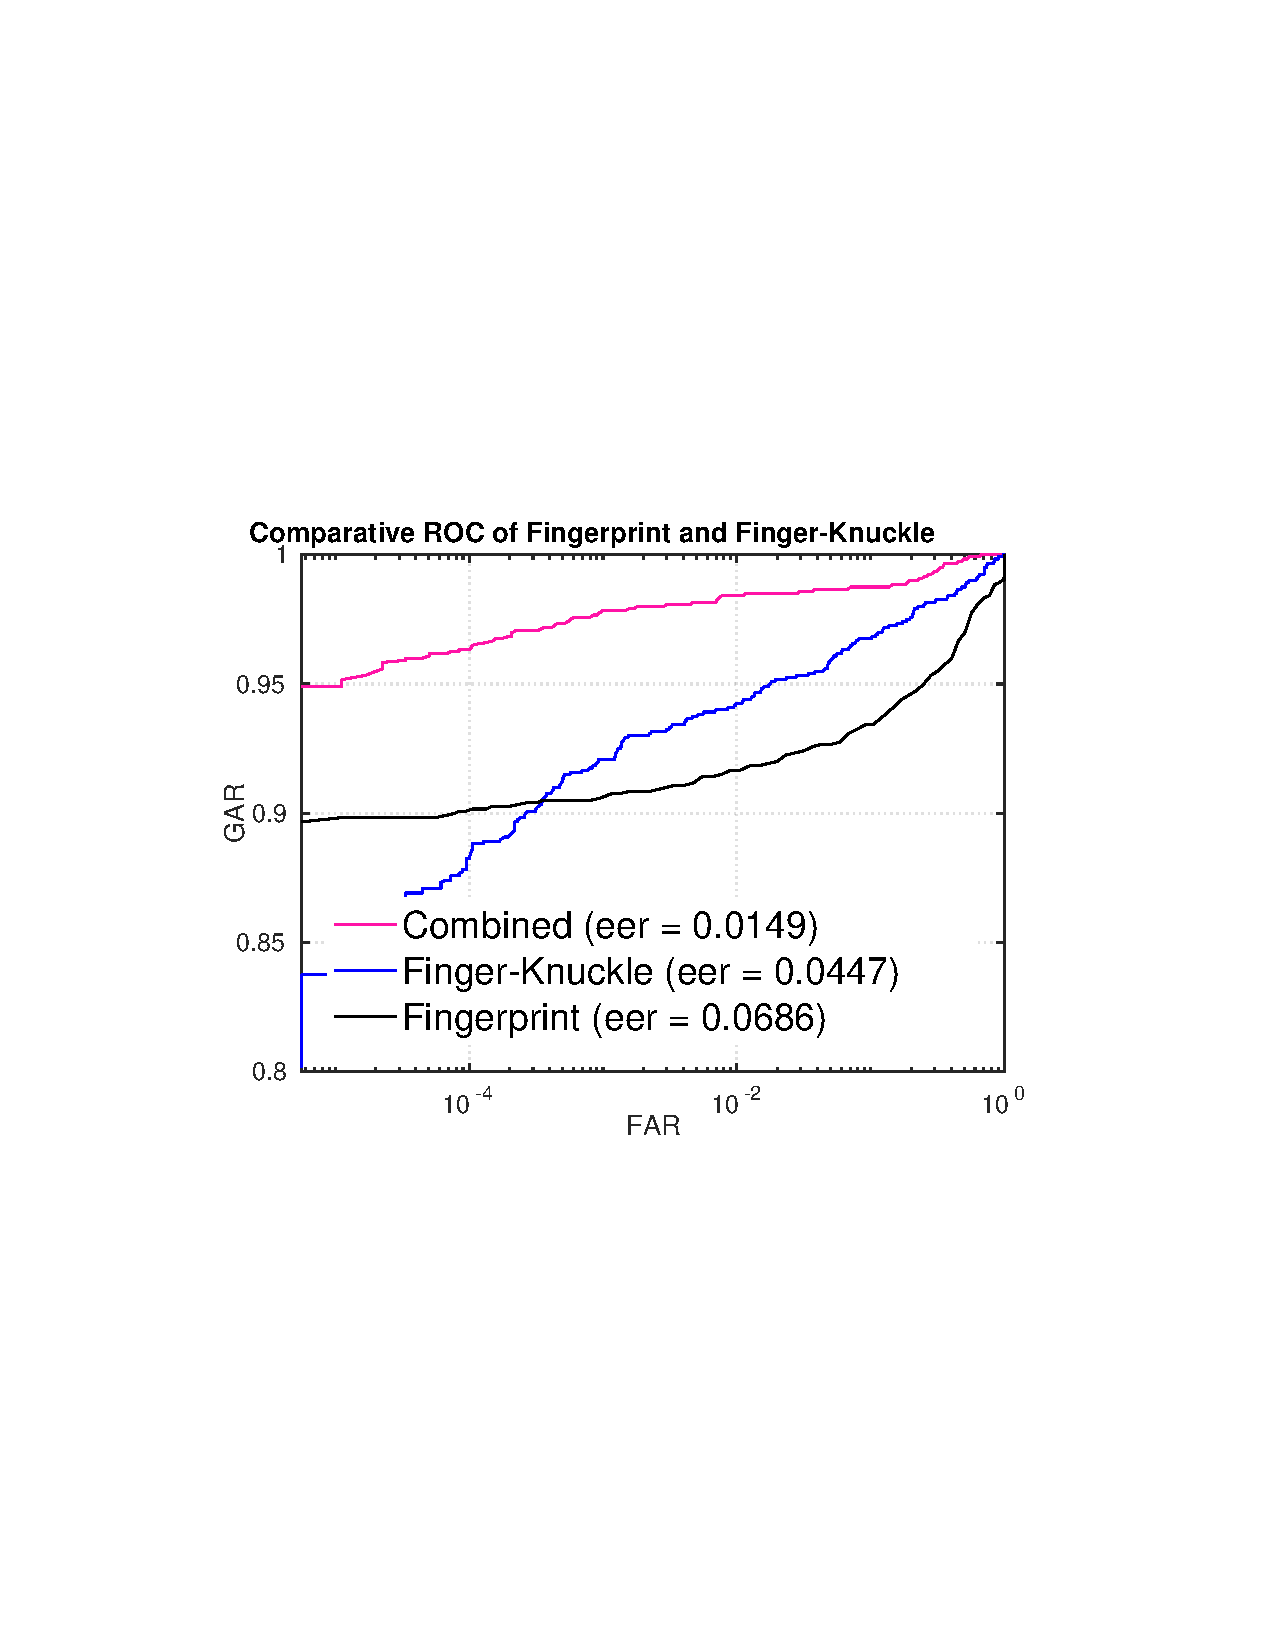
\includegraphics[width=2in]{Figures/dynamic/01.pdf}
    \label{}}
    \subfloat[]{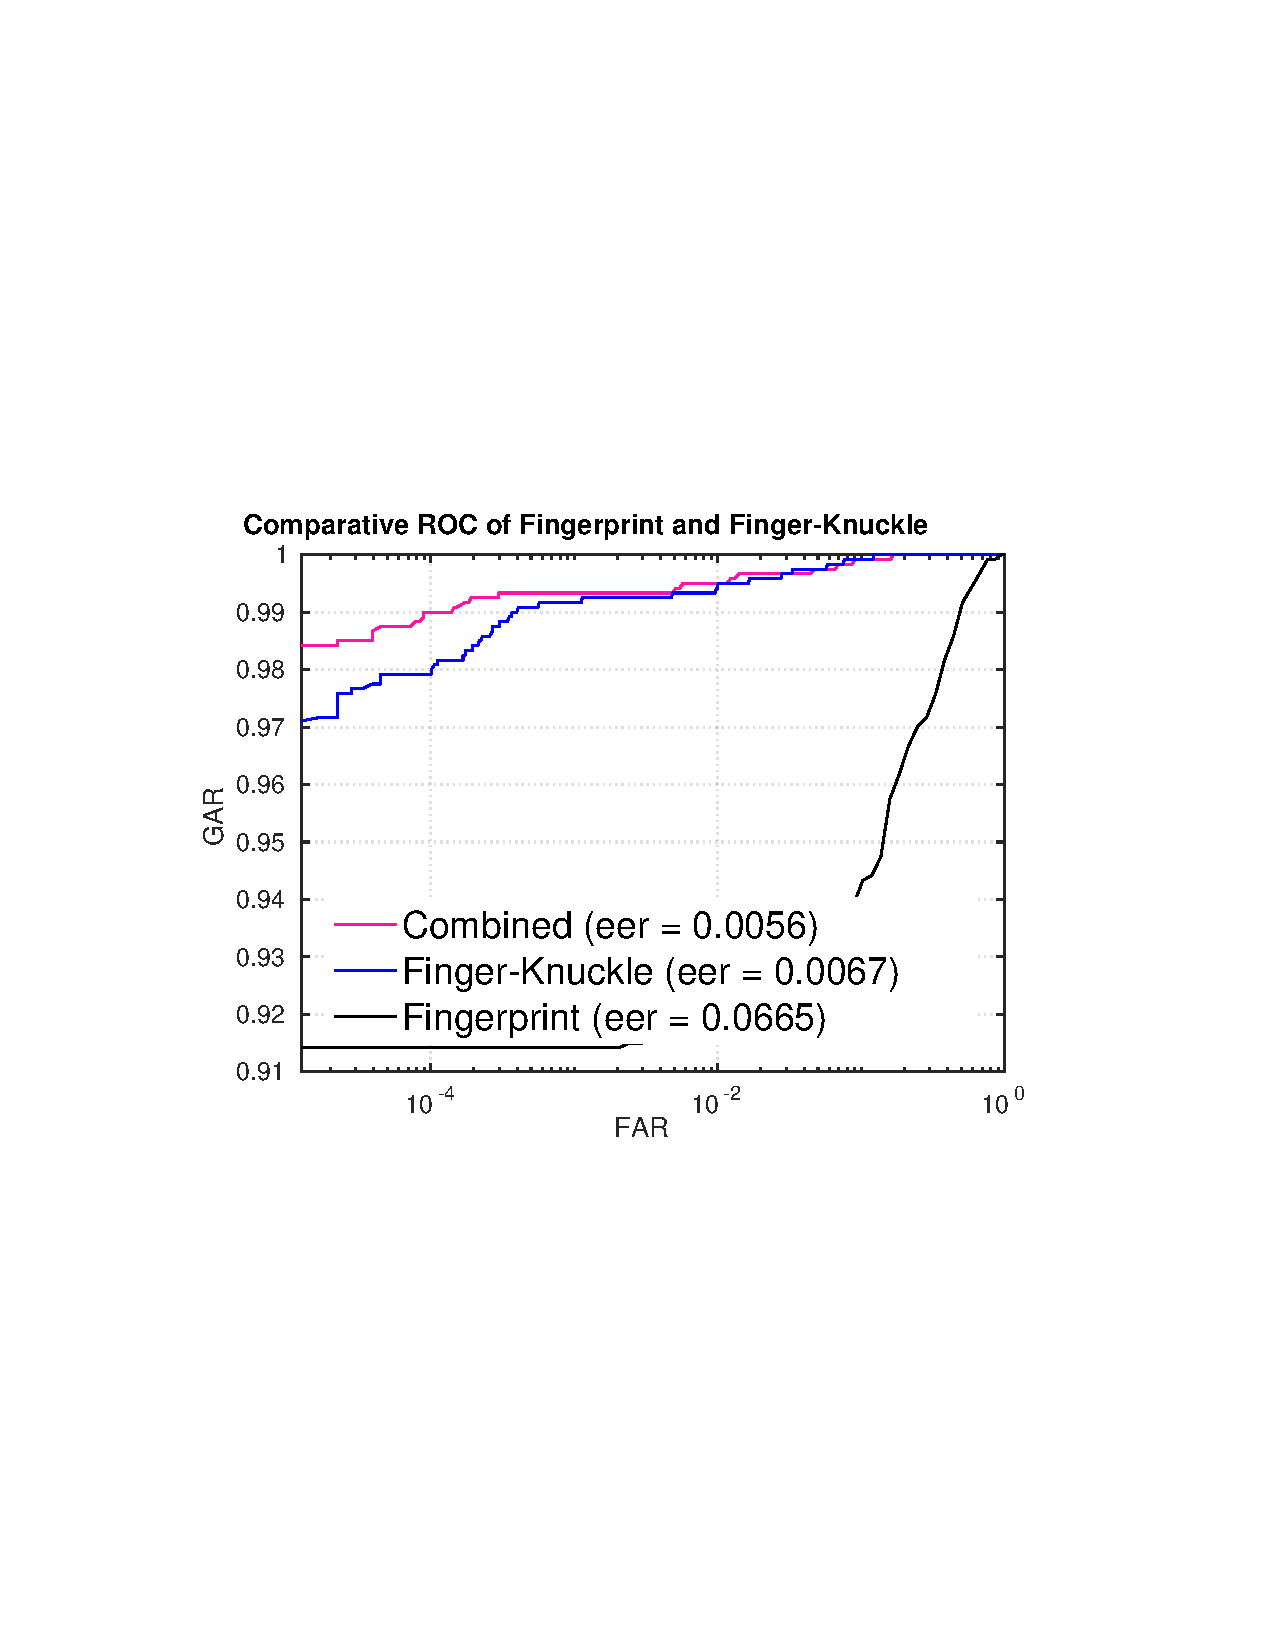
\includegraphics[width=2in]{Figures/dynamic/02.pdf}
    \label{}}
    \subfloat[]{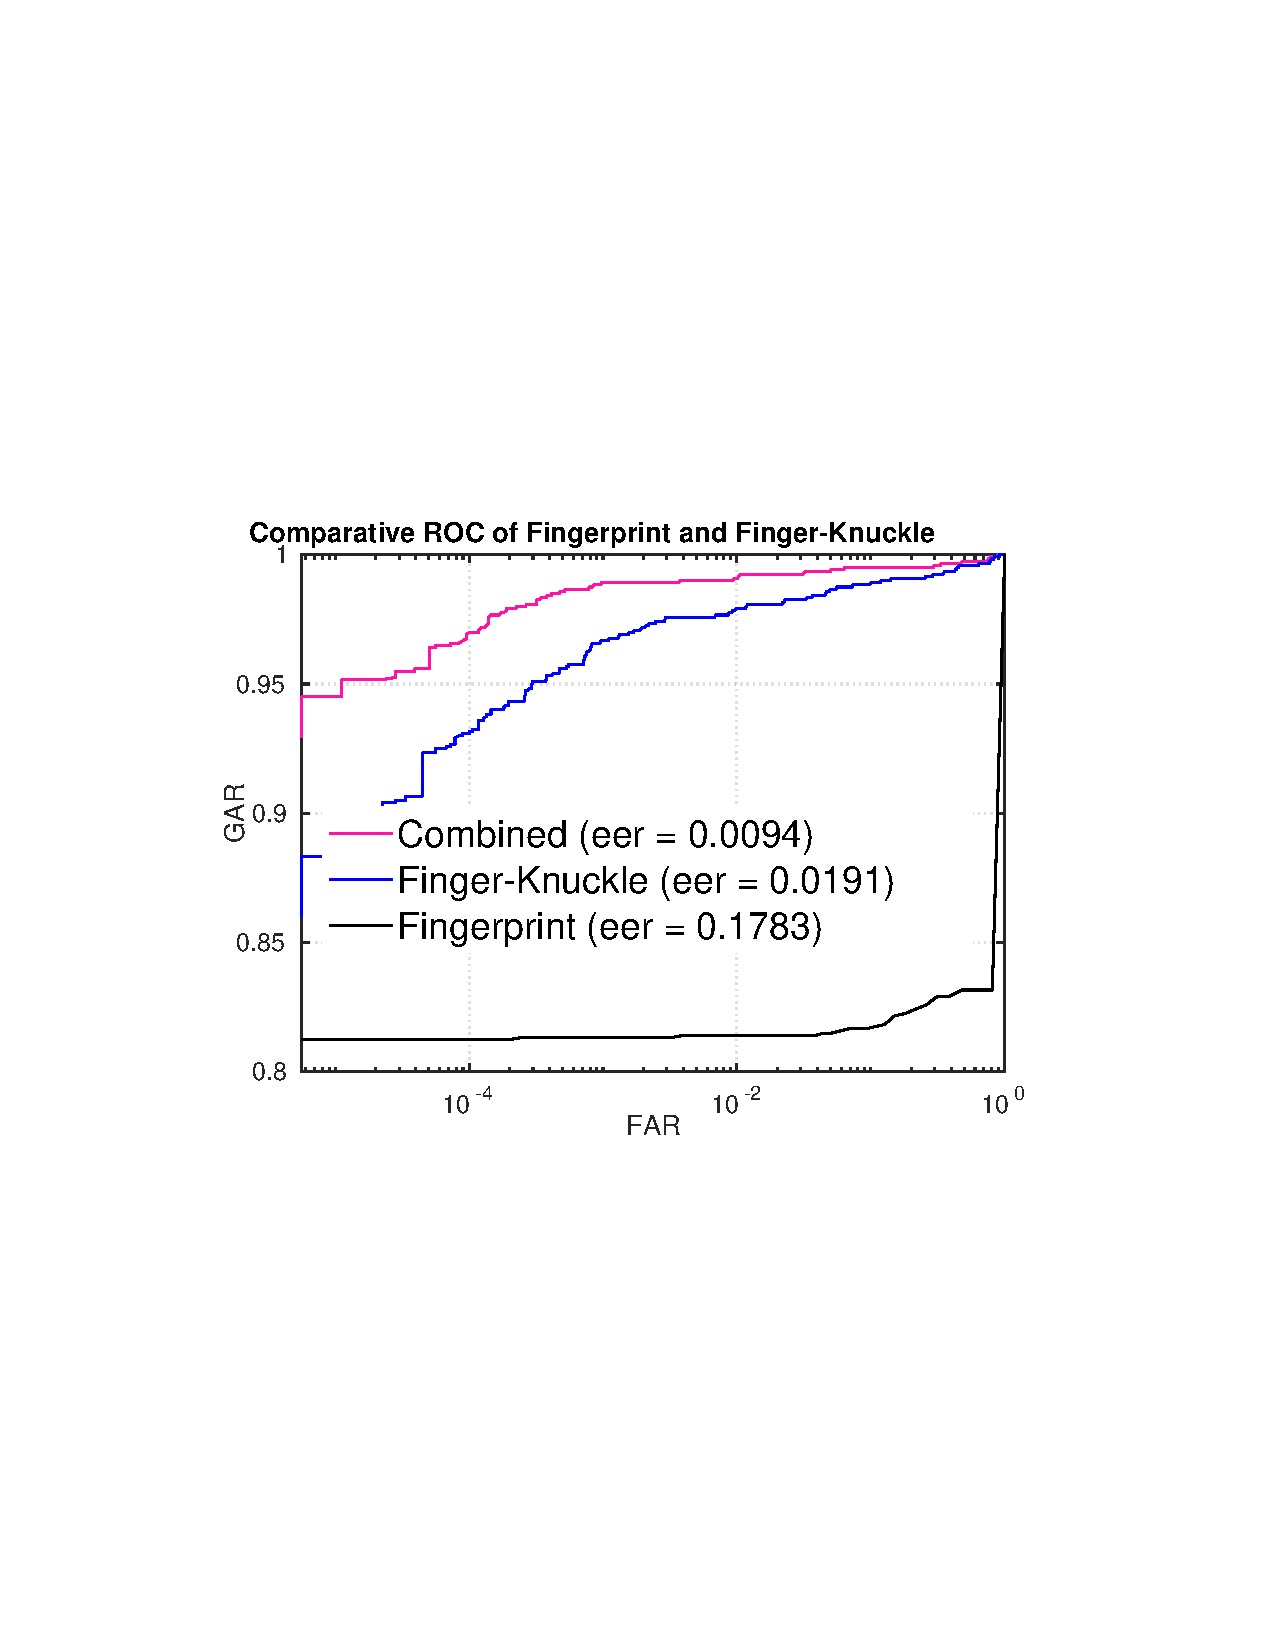
\includegraphics[width=2in]{Figures/dynamic/04.pdf}
    \label{}}

    \subfloat[]{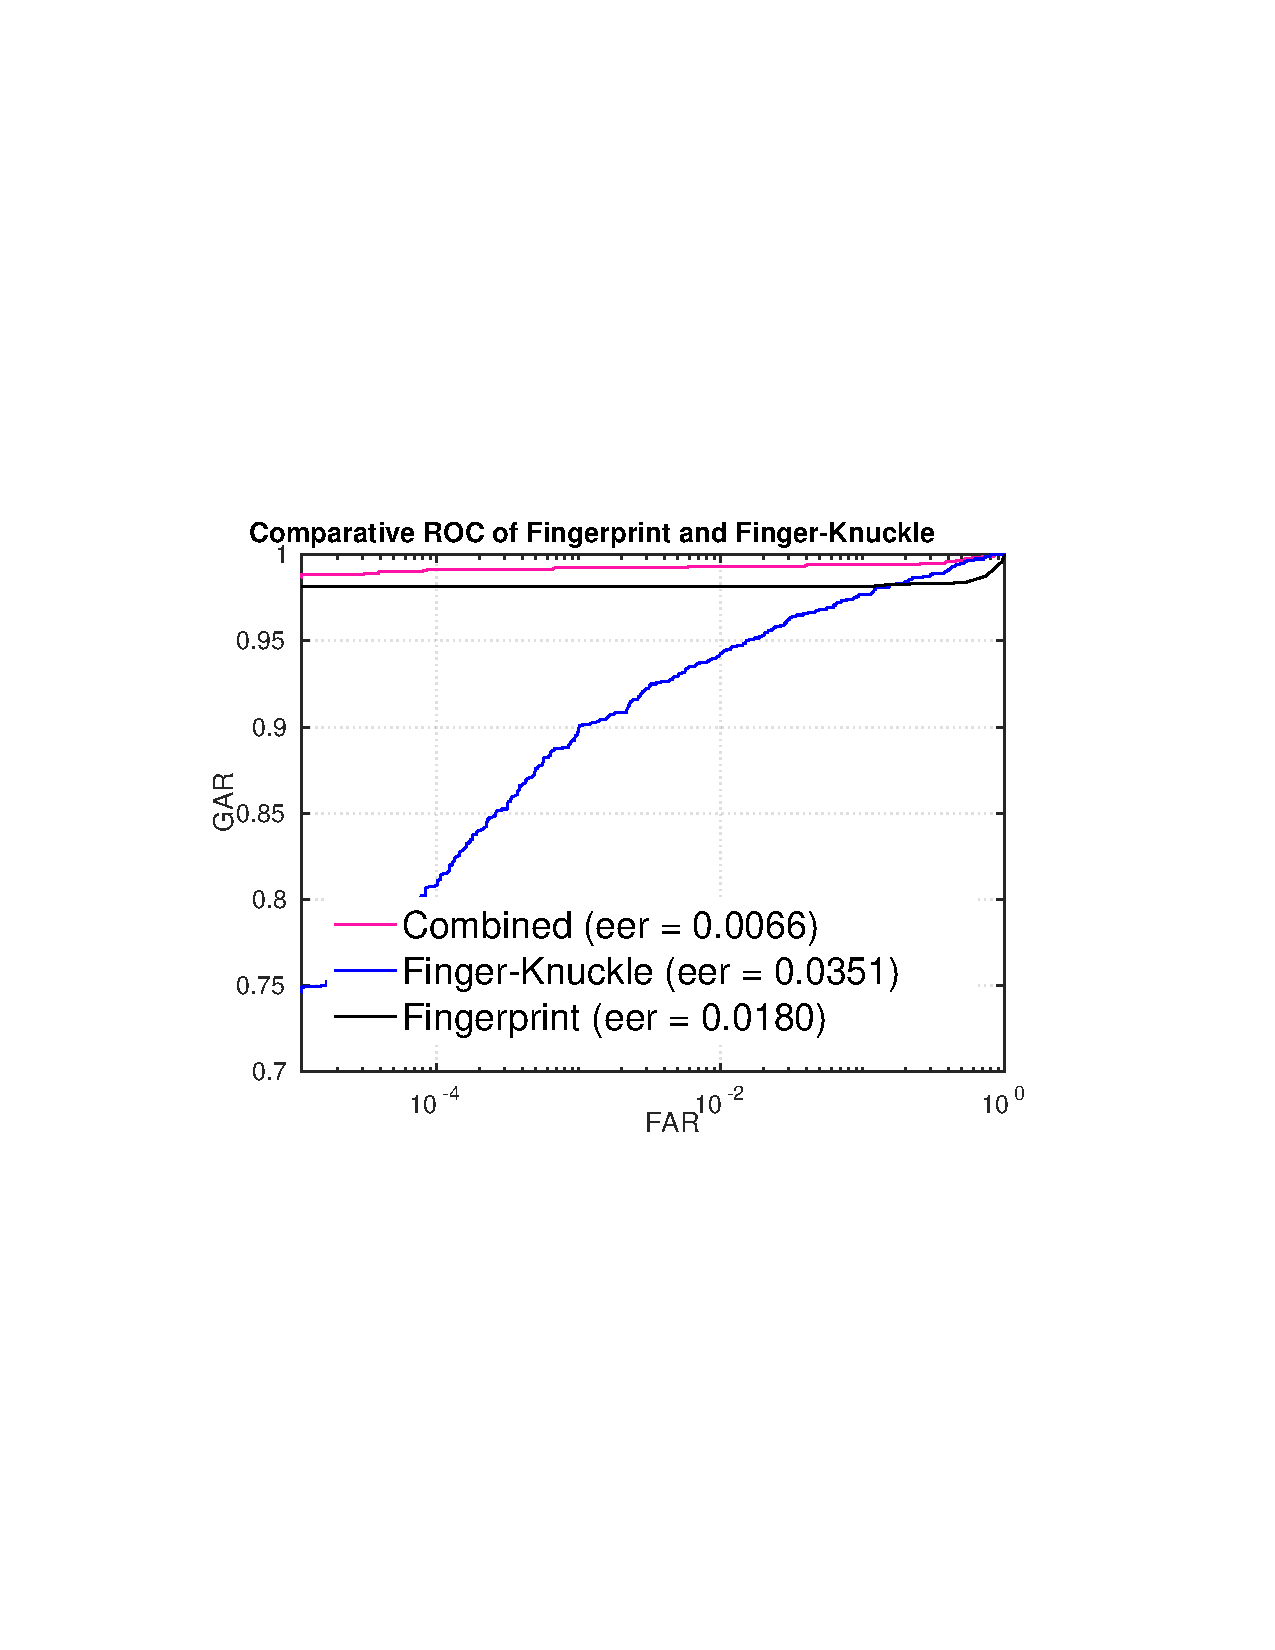
\includegraphics[width=2in]{Figures/dynamic/05.pdf}
    \label{}}
    \subfloat[]{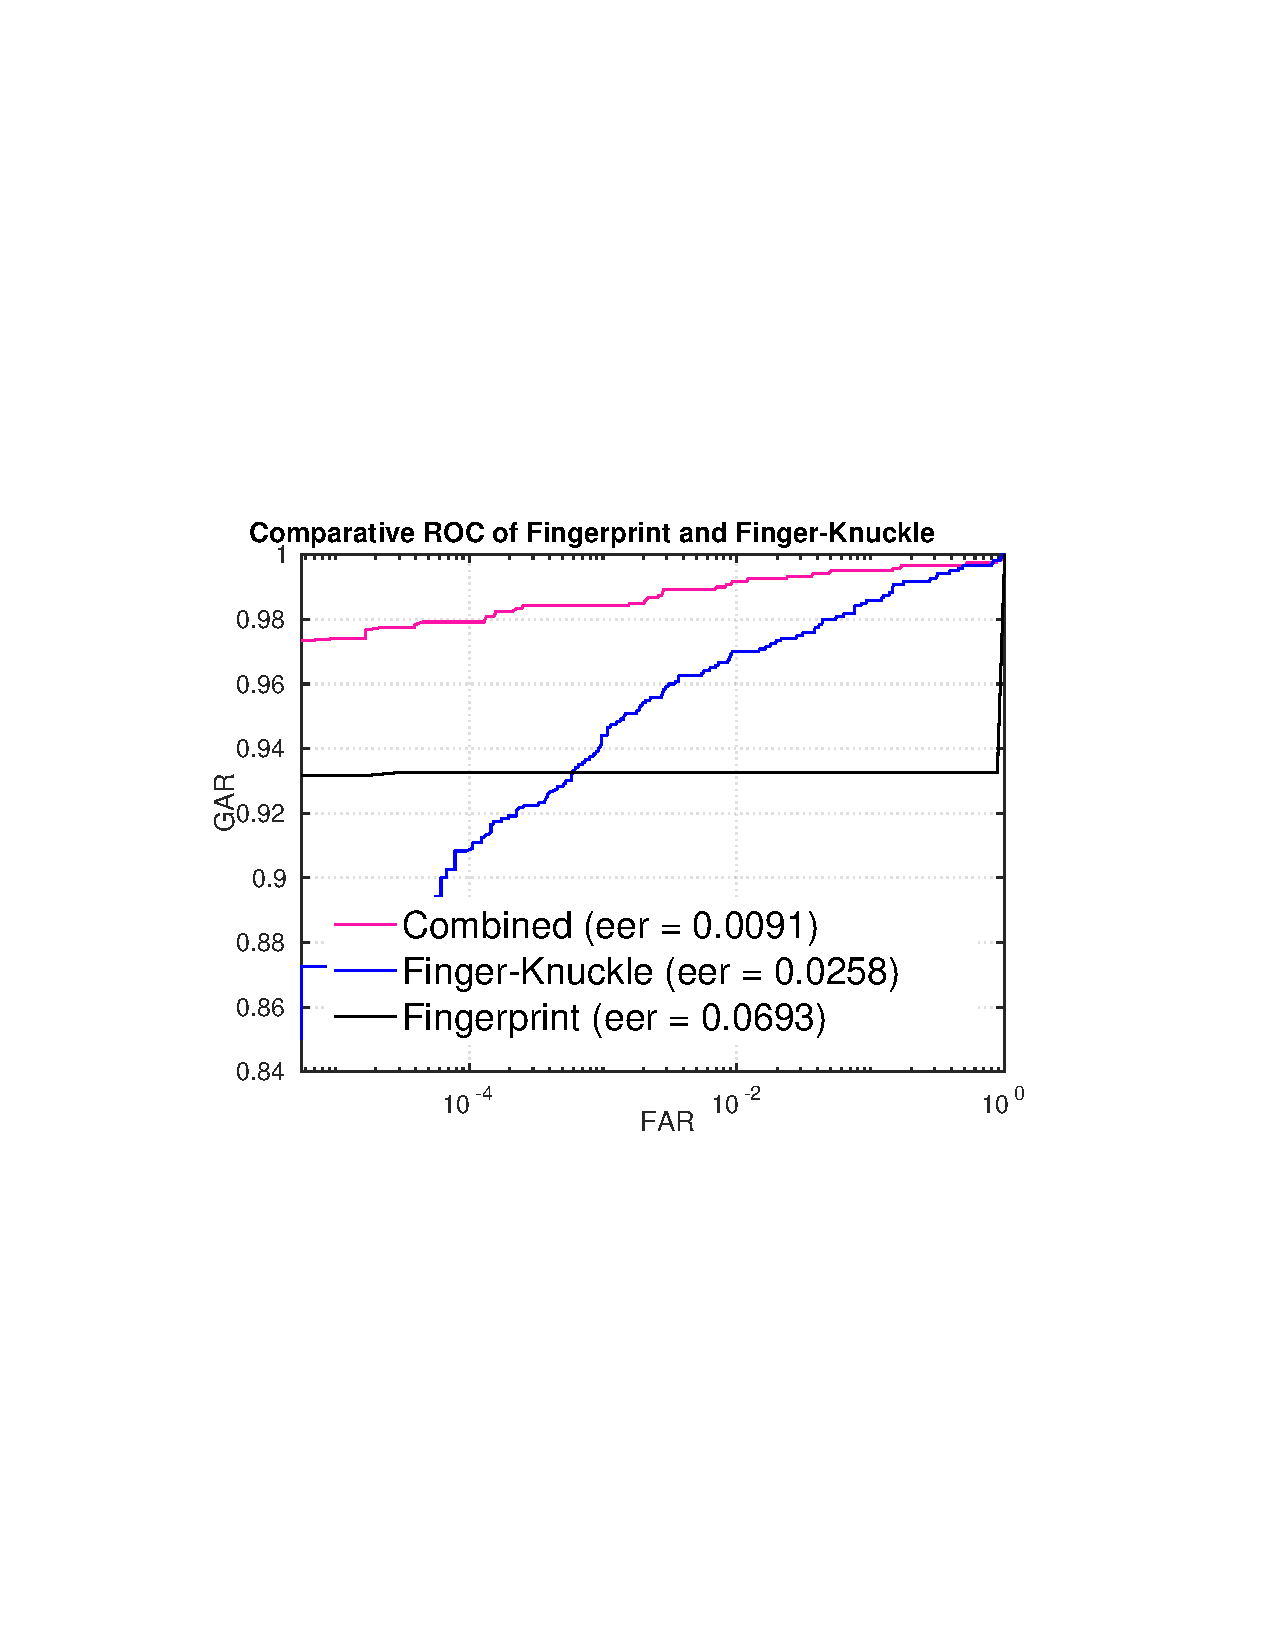
\includegraphics[width=2in]{Figures/dynamic/06.pdf}
    \label{}}
    \subfloat[]{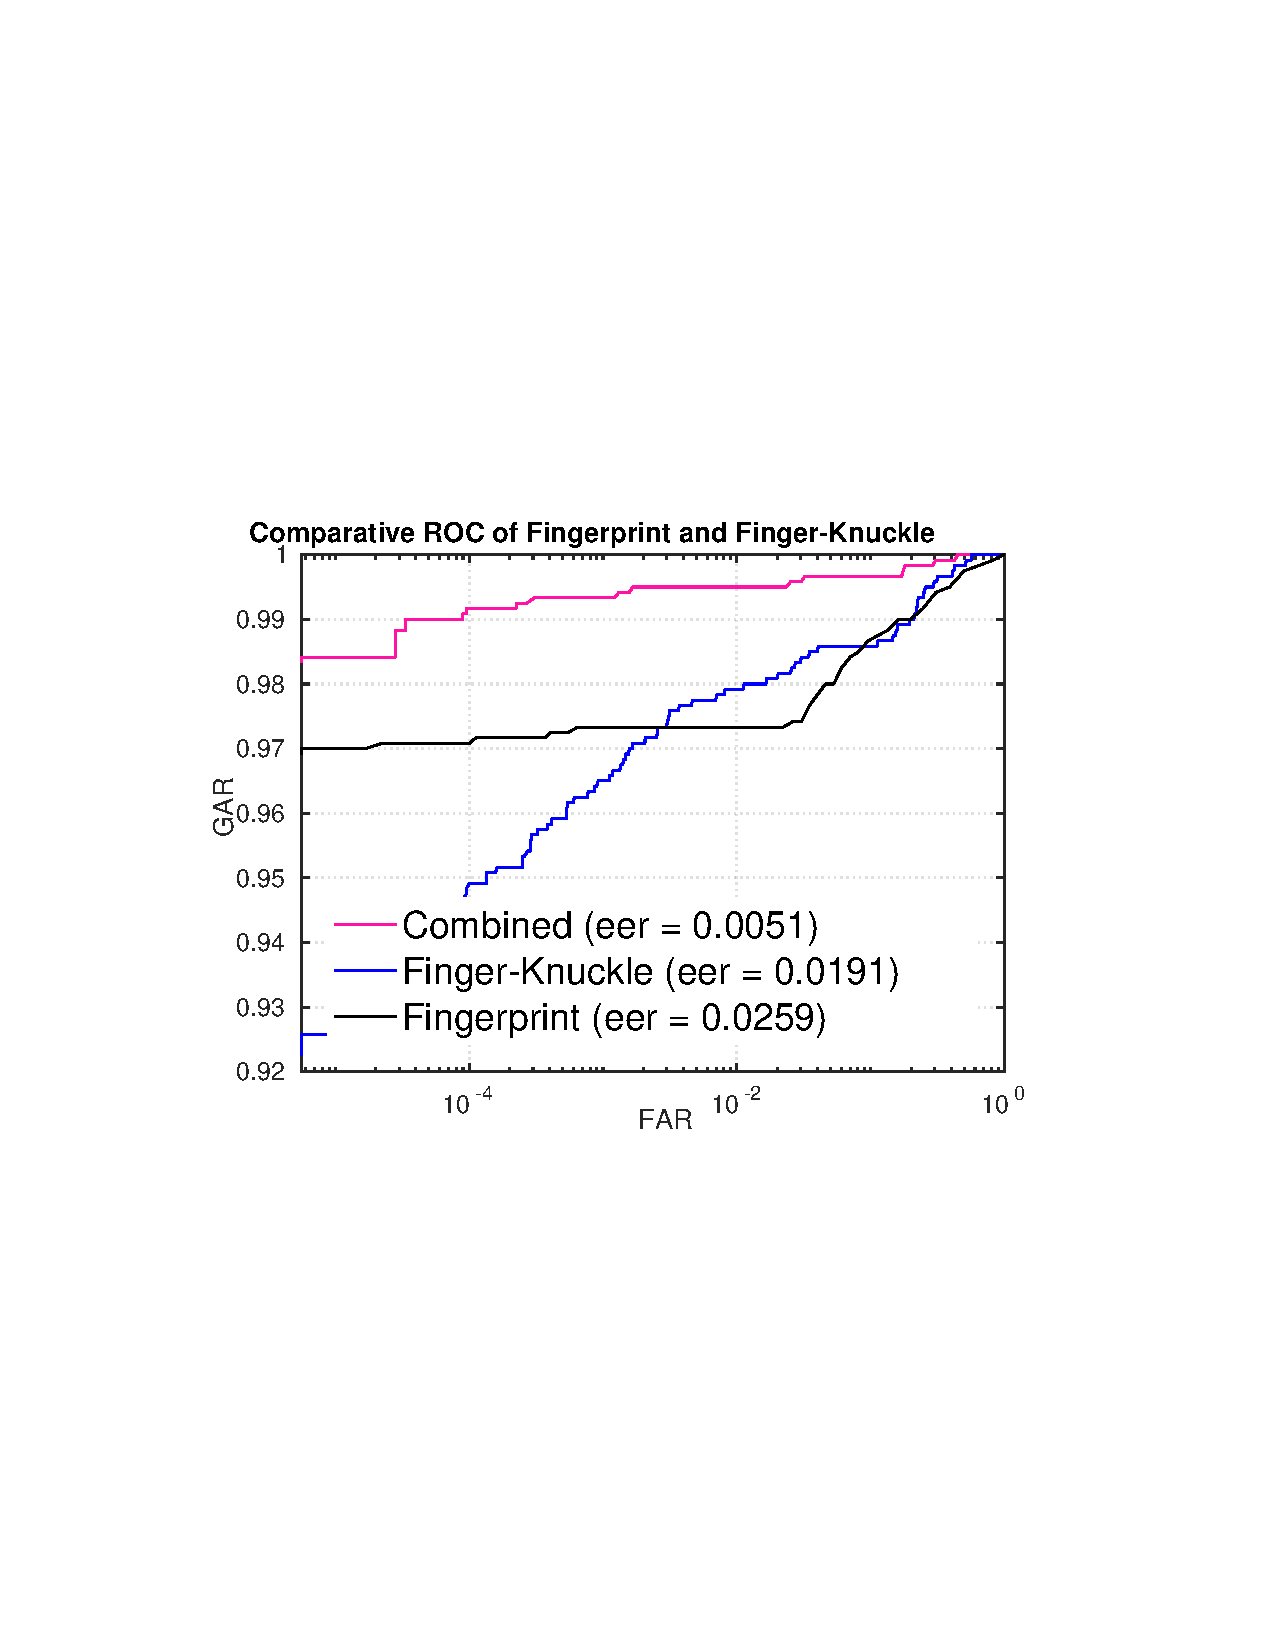
\includegraphics[width=2in]{Figures/dynamic/07.pdf}
    \label{}}

    \subfloat[]{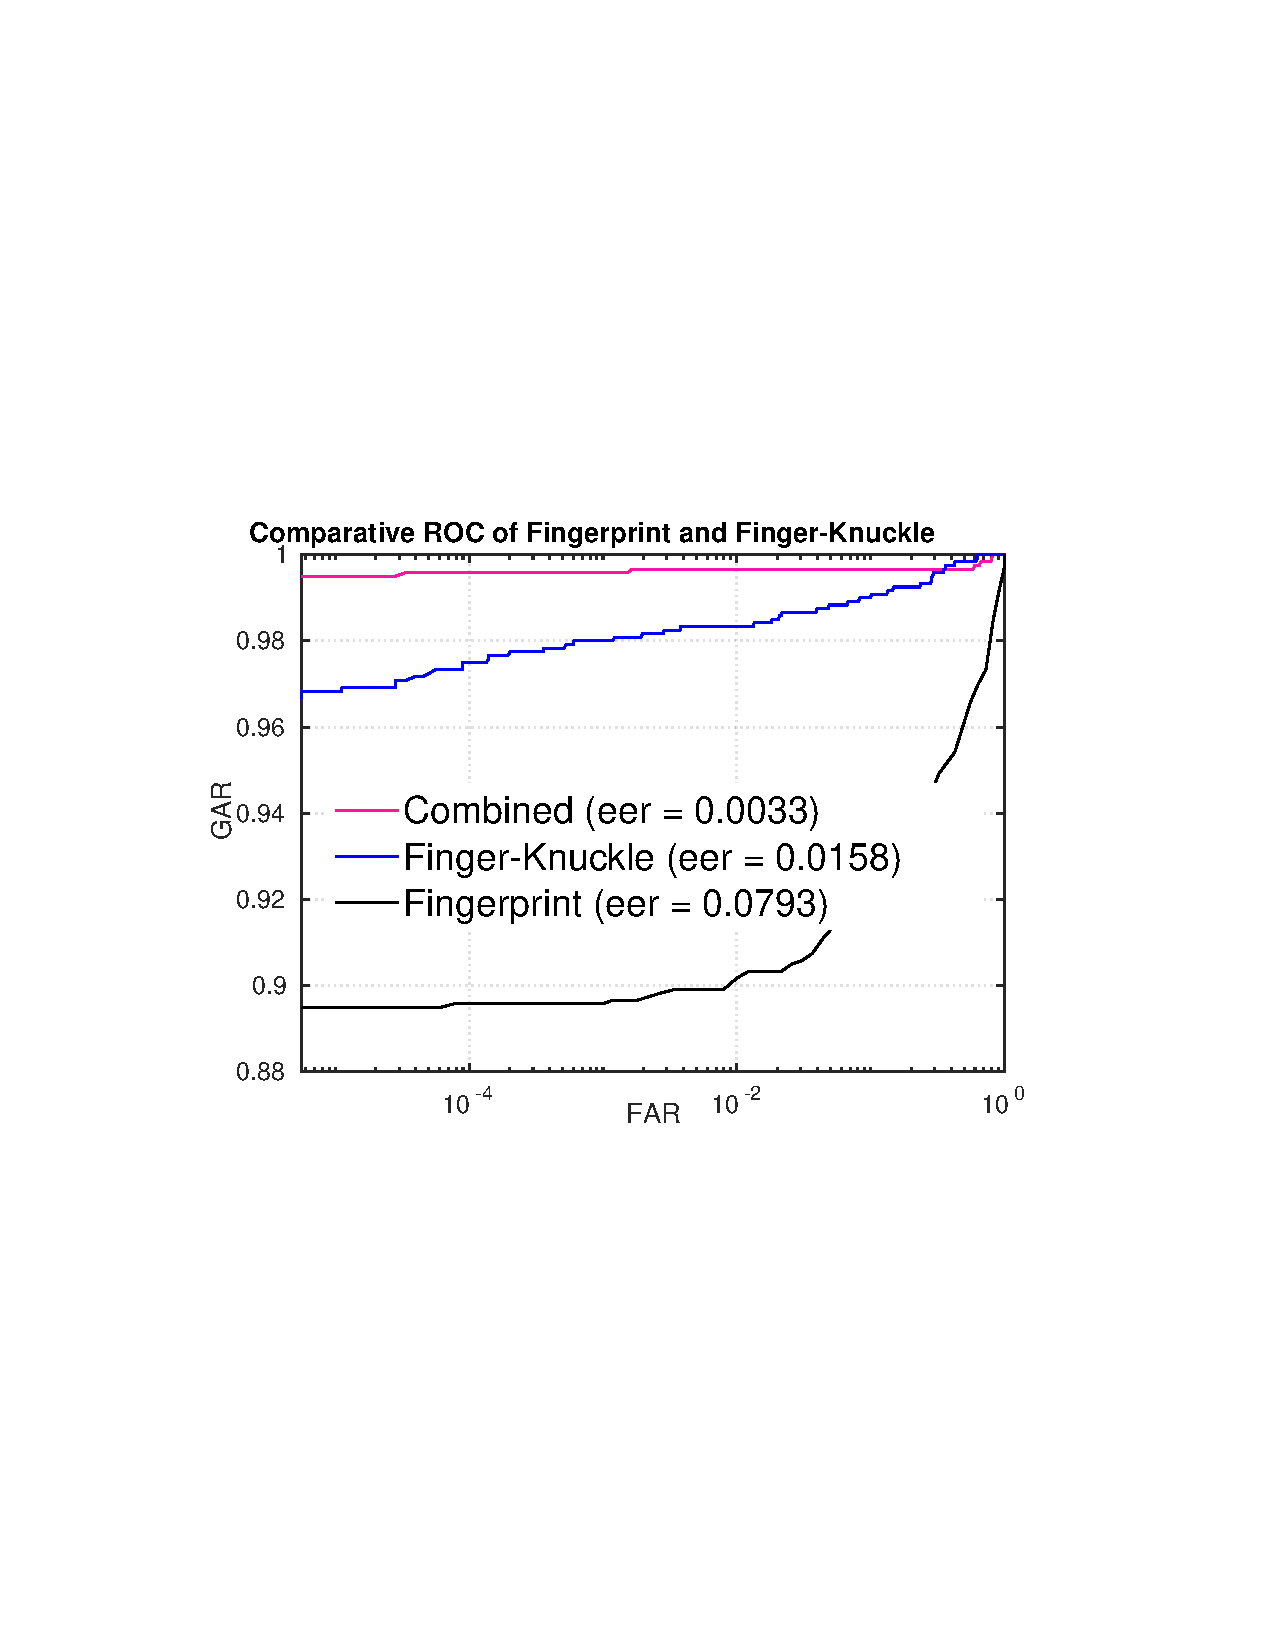
\includegraphics[width=2in]{Figures/dynamic/08.pdf}
    \label{}}
    \subfloat[]{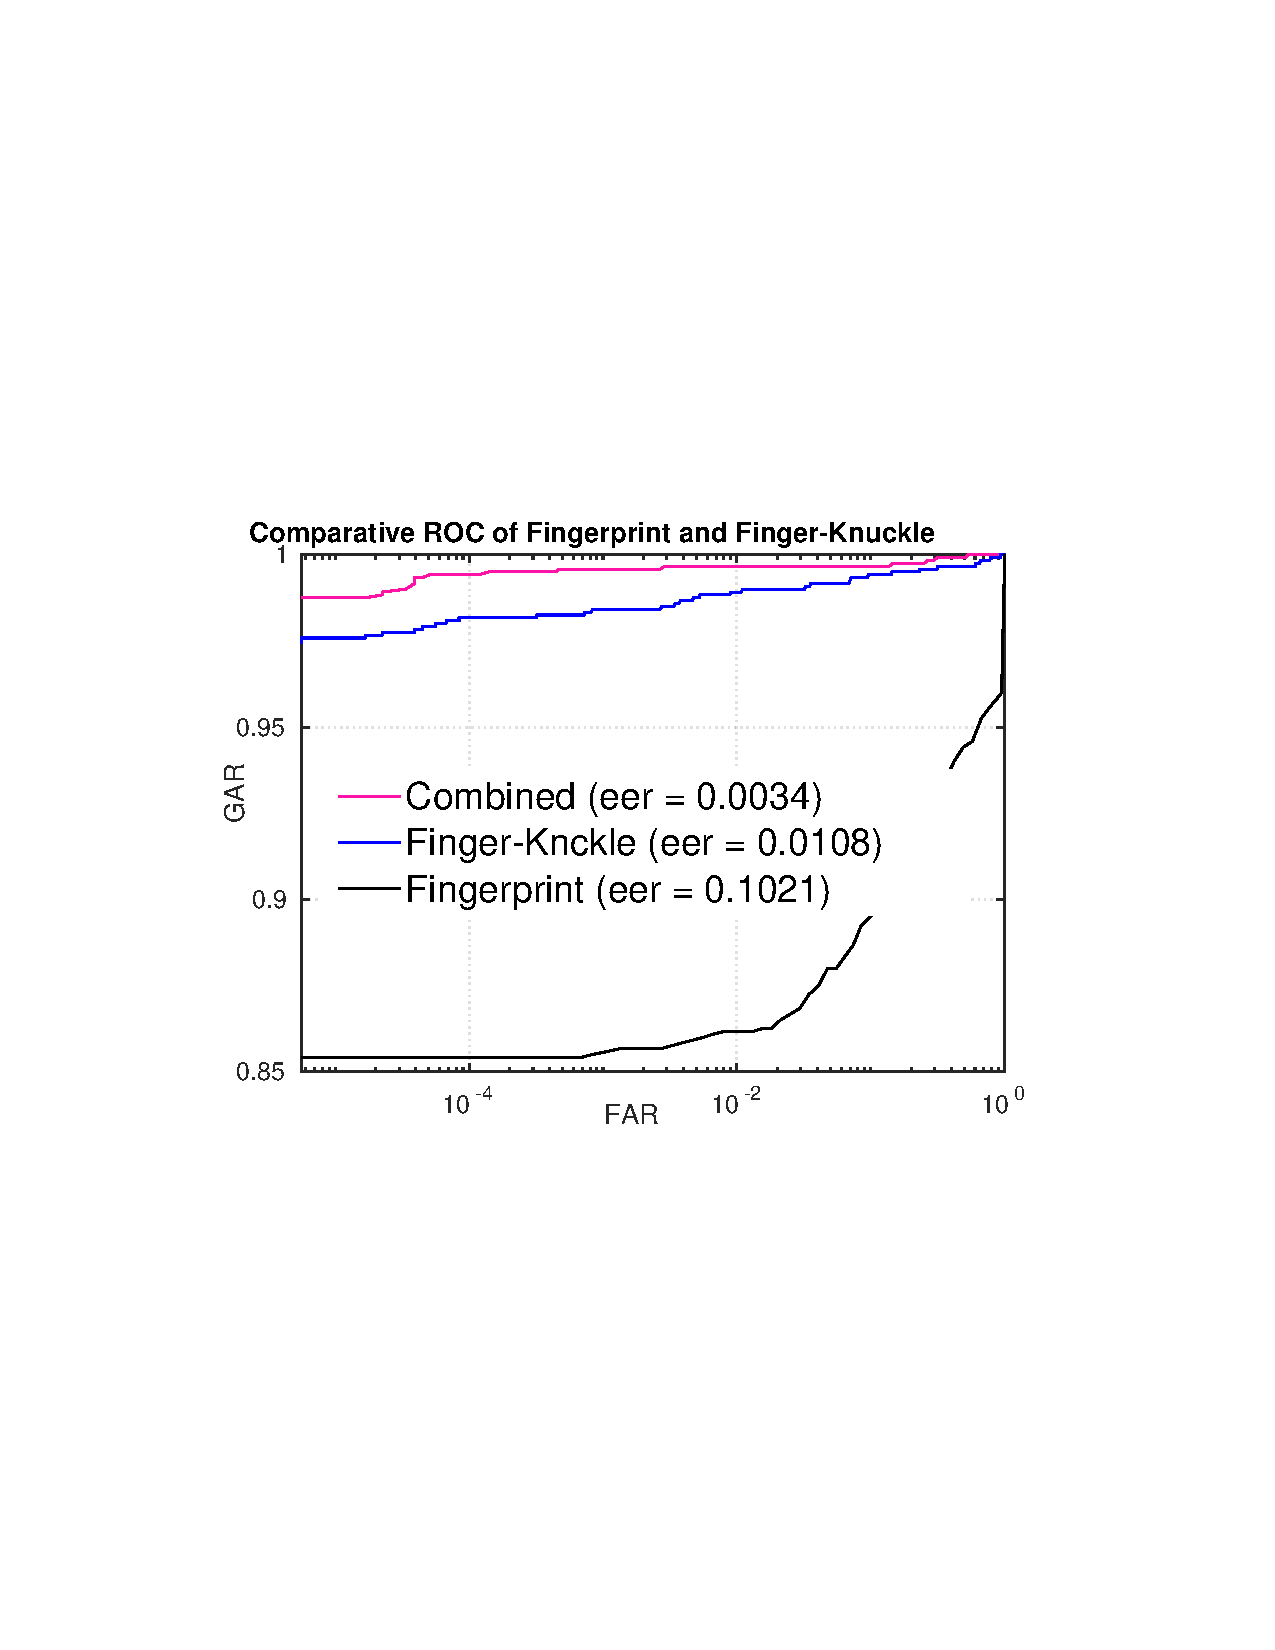
\includegraphics[width=2in]{Figures/dynamic/09.pdf}
    \label{}}
    \subfloat[]{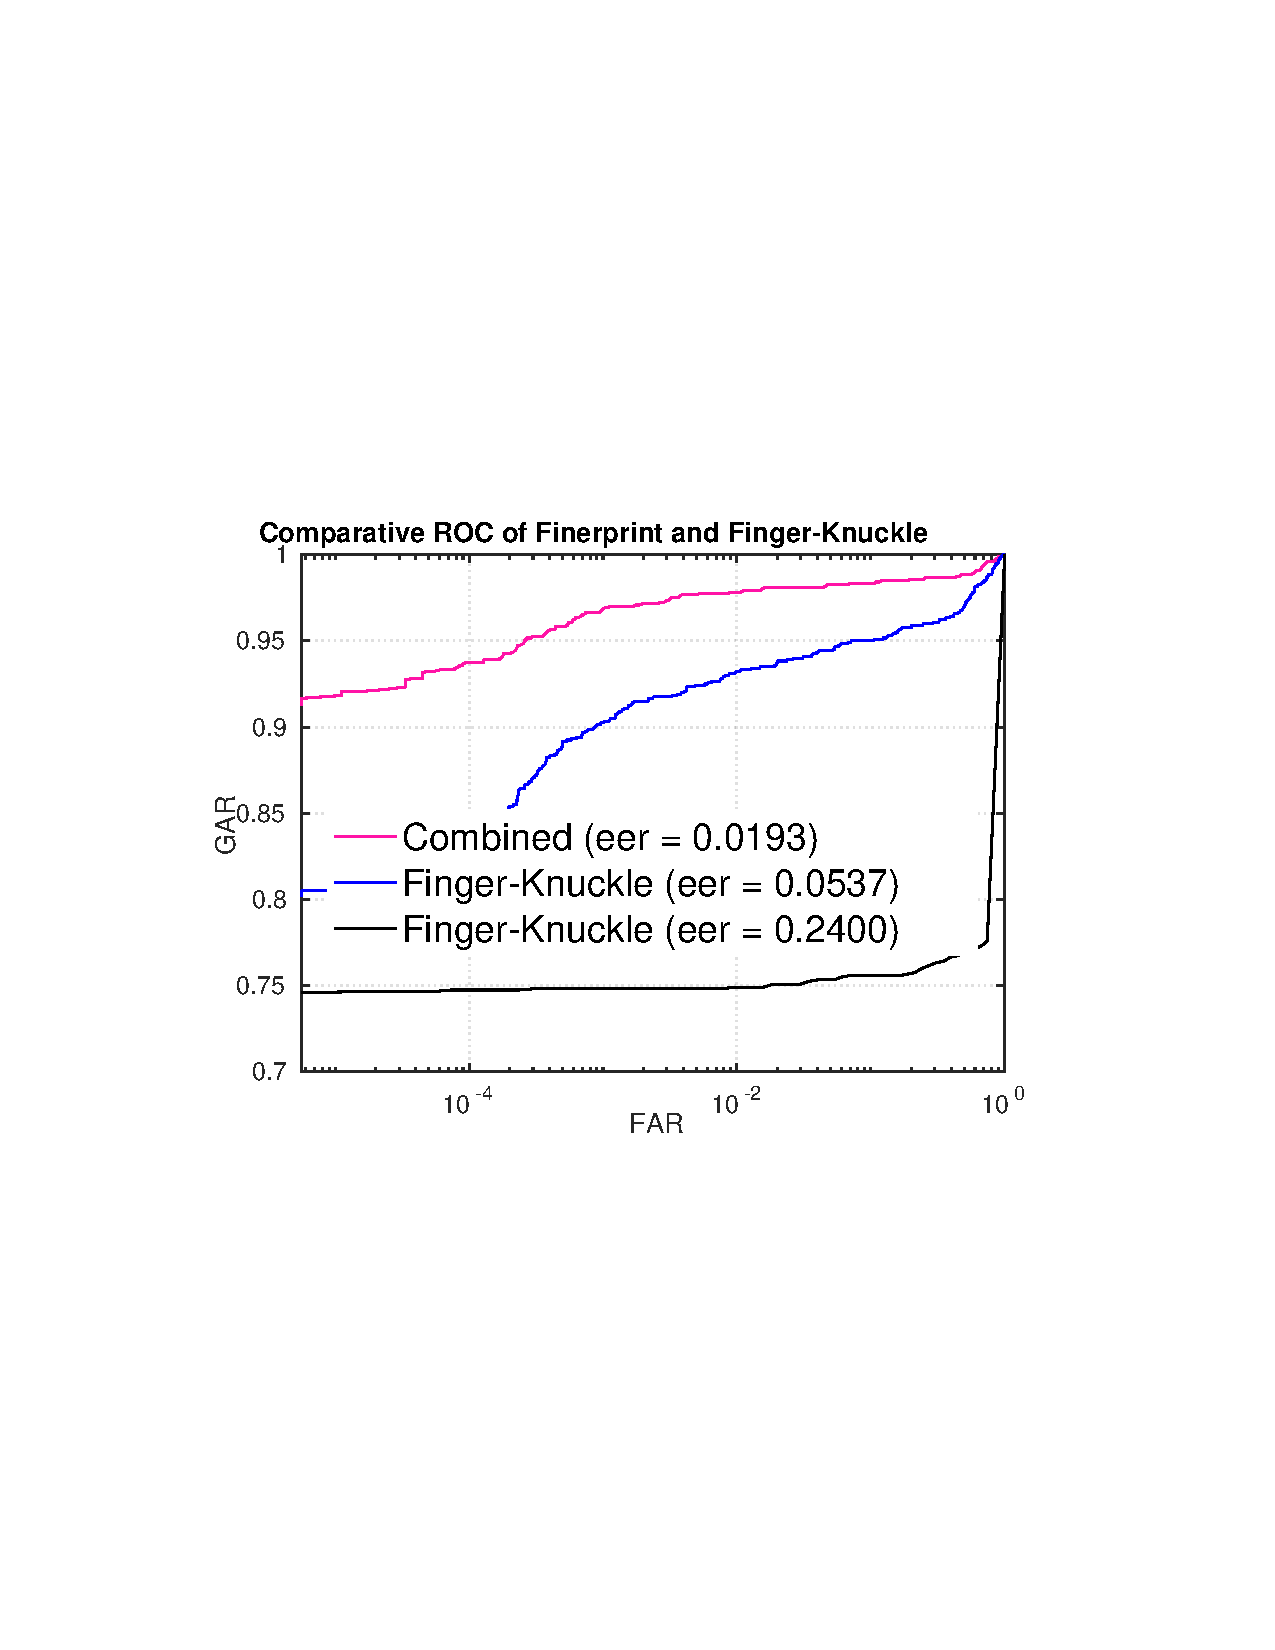
\includegraphics[width=2in]{Figures/dynamic/10.pdf}
    \label{}}
    \caption{Comparative performance the simultaneously acquired fingerprint and finger knuckle images. The figures on these (a)-(d) indicate ROC from the left-hand fingers, and figures on these (e)-(i) indicate ROC from the right hand fingers. The figures from top to bottom row presents the ROC from the little finger in (a), ring finger in (b), index finger in (c), and thumb in (d) of left hand, While the thumb in (e), index finger in (f), middle finger in (g),  ring finger in (h), and little finger in (i) of right hand.}
    \label{joint-performance}
\end{figure*}

The combined performance from the simultaneously acquired finger knuckle and fingerprint images is shown in Fig. \ref{joint-performance}. Table \ref{fusion-eer} presents a summary of respective EER values from each of the nine fingers, both individually from the finger knuckle or fingerprint and their combination. It can be observed from these figures and table that performance improvement from the joint usage of two biometric is quite significant except for the thumbprints. The performance from the fingerprint images acquired from the thumbs is already quite high which can limit the effectiveness for simultaneously acquired finger knuckle images. The results presented in Fig. \ref{joint-performance} indicates that the extent of the performance improvement varies for the different fingers. Fig. \ref{score-distribution} illustrates the distribution of match score for the two sample fingers in our database. It can be observed from this figure that the distribution of match scores, from the two simultaneously acquired images, is quite distinct for the two classes. Therefore, the joint usage of such match scores is expected to offer more reliable user authentication.

\begin{table}[ht]
    \centering
    \caption{Relative EER values for the fingerprint and finger knuckle images.}
    \begin{tabular}{cccc}
    \hline
    Finger       & Finger Knuckle & Fingerprint & Combined \\ \hline
    Left Little  & 0.0447        & 0.0686     & 0.0149  \\
    Left Ring    & 0.0067        & 0.0665    & 0.0056  \\
    Left Index   & 0.0191        & 0.1783     & 0.0094  \\
    Left Thumb   & 0.0351        & 0.0180     & 0.0066  \\
    Right Thumb  & 0.0258        & 0.0693     & 0.0091  \\
    Right Index  & 0.0191        & 0.0259     & 0.0051  \\
    Right Middle & 0.0158        & 0.0793     & 0.0033  \\
    Right Ring   & 0.0108        & 0.1021     & 0.0034  \\
    Right Little & 0.0537        & 0.2400     & 0.0193  \\ \hline
    \end{tabular}
    \label{fusion-eer}
\end{table}


\begin{figure}[ht]
    \begin{center}
        \subfloat[]{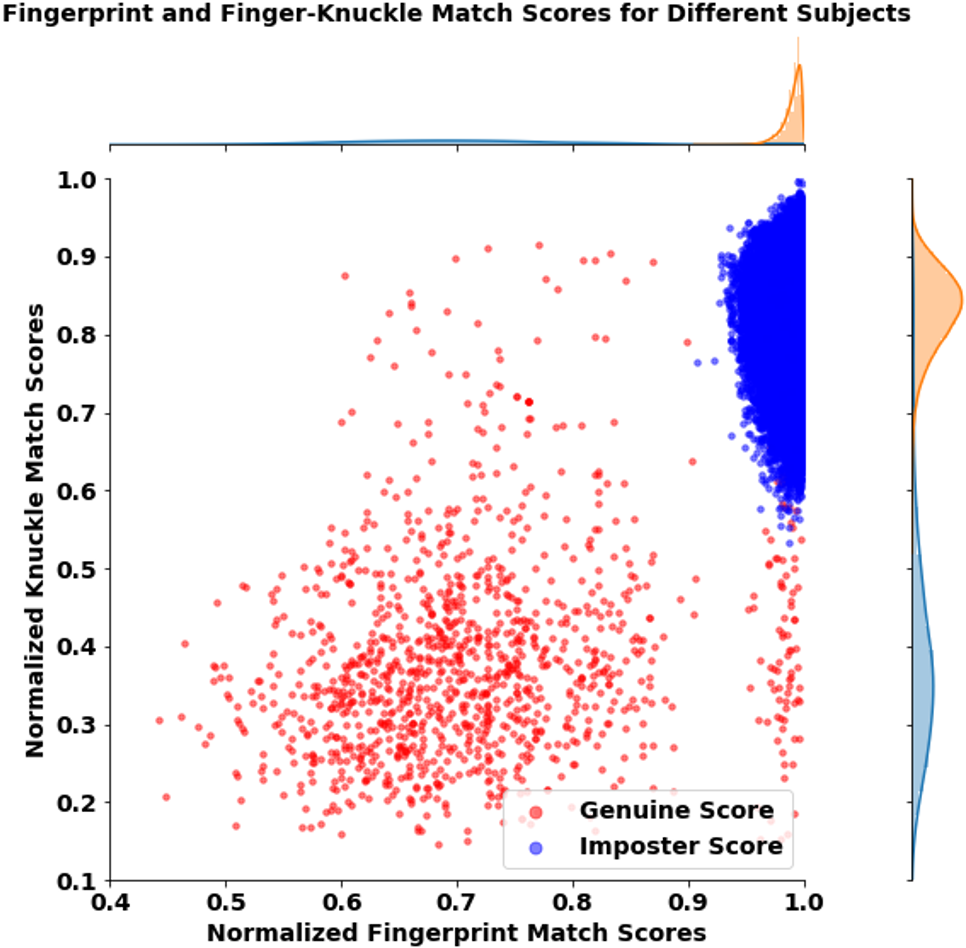
\includegraphics[width=1.65in]{Figures/score-distribution-a.png}
        \label{}}
        \subfloat[]{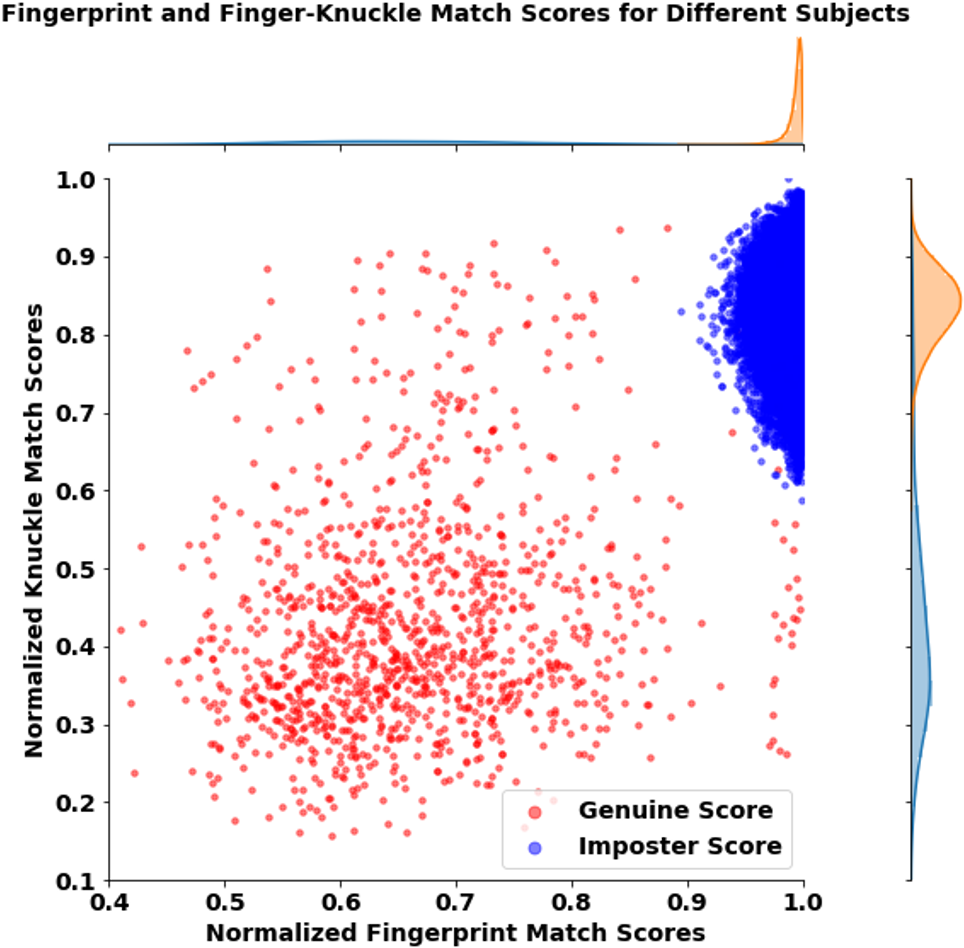
\includegraphics[width=1.65in]{Figures/score-distribution-b.png}
        \label{}}
    \end{center}
    \caption{Distribution of finger-knuckle and fingerprint match scores for two sample fingers: (a) left hand ring finger and (b) right hand index finger.}
    \label{score-distribution}
\end{figure}